\section{Methodology}
\subsection{Description of Data Sources}
\subsubsection{Central Insolvency Register}
\paragraph{Data suppliers}
The CIR \cite{rechtspraak:1} is operated by the Dutch government and contains company insolvency data supplied by the courts and the administrators. Courts are obliged to supply the insolvency data and free consultation thereof according to the insolvency law, article 19 \cite{law:1}. CIR started the digital register on the 1st of January 2005 and retains insolvency cases until six months after the ending of the insolvency. CIR also contains other data such as personal debt restructuring (\textit{schuldsanering}), personal insolvency and company's failure to pay (\textit{surseance}) but this data is out of scope.

\paragraph{Entity records}
The CIR register contains the following entities in numbers of records (as of 2019-03-21):

\begin{table}[h]
\caption{number of entity records.}
\centering
\begin{tabular}{l r r}
\hline\hline
Entity & no. of records\\
\hline
Court & 11 \\
Supervisory Judge (distinct names) & 580 \\
Insolvency & 51,392 \\
Administrator (distinct names) & 58,201 \\
Publication & 142,172 \\
Report & 357,803 \\
... progress report & 237,657 \\
... financial attachment. & 120,146 \\
\hline
\end{tabular}
\label{table:cir_contents}
\end{table}

Publications on an insolvency case are done by the court and include the initial declaration of bankruptcy. Administrators periodically submit progress reports as well as financial attachments to the CIR.

\paragraph{Entity identifiers}
The web service response in XML is semi structured data. It provides natural unique identifiers for Insolvency Cases, Publications and Reports	so they can be easily stored in normalized SQL tables and linked. The other entities: Courts, Judges and Administrators have no identifiers but consist of free text fields for their name parts. These entities must be de-duplicated en linked to a master data record. It can be easily observed in table \ref{table:cir_contents} that this is certainly needed for administrators \todo[inline]{state estimated number of administrators}.

\paragraph{Entity relations}
Figure \ref{fig:cir-erd} below shows the relationships between the entities including their cardinality. Note that some relationships are time dependent, e.g. a judge can be replaced during the lifetime of an insolvency case. Since 1-1-2019 there can be two judges appointed to one case.

\begin{figure}[h]
	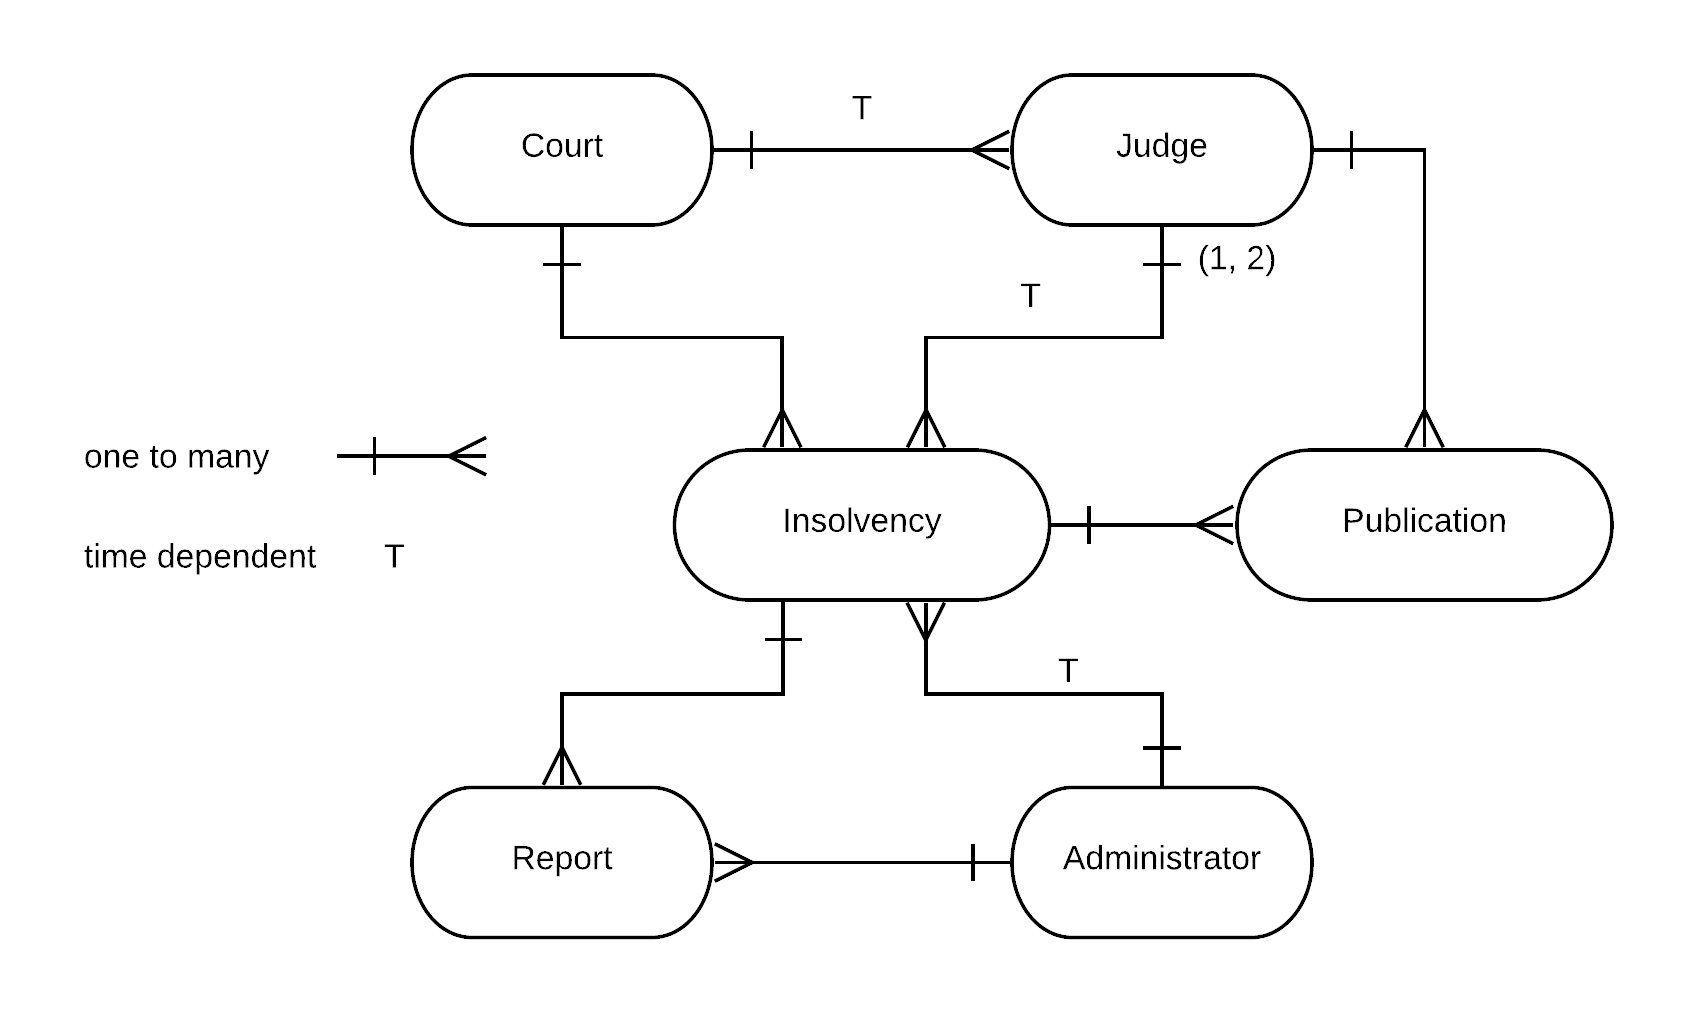
\includegraphics[width=1\linewidth]{images/cir_erd_2.png}
	\caption{Insolvency entity relations.}
	\label{fig:cir-erd}
\end{figure}

\paragraph{Administrator Reports}
A second web service operated by CIR provides administrator reports in PDF format. These reports hold much of the unstructured data. Recofa has published templates for both progress and financial attachment reports \cite{rechtspraak:3} which provide a certain structure to the contents.

\subsubsection{Register of lawyers, NOvA Tableau}\label{NOvA Tableau}
The NOvA tableau is the official register for lawyers and maintained by the \textit{Nederlandse Orde van Advocaten (NOvA)}\cite{nova:1}. Lawyers are obliged to be registered in the tableau by the lawyer's law (\textit{advocatenwet}, article 1 \cite{law:2}). NOvA offers an on-line search form where keyword search and filters can be applied to search for a lawyer. This data source was chosen to collect the master data for Administrators. 

\subsubsection{Register of judges, Nevenfuncties van rechters}\label{Nevenfuncties Rechters}
The Register for ancillary positions for judges is made available by \textit{de Rechtspraak}\cite{rechtspraak:2}. It offers an on-line form and returns the name, current and historical occupation and ancillary positions. This data source was chosen to collect the master data for Judges.

\subsection{Information System Description}
Figure \ref{System overview} gives an overview of the system components for sourcing, extracting, enriching and integrating the  data and making the resulting structured and higher level information available to the user's analysis.

\begin{figure}[h]
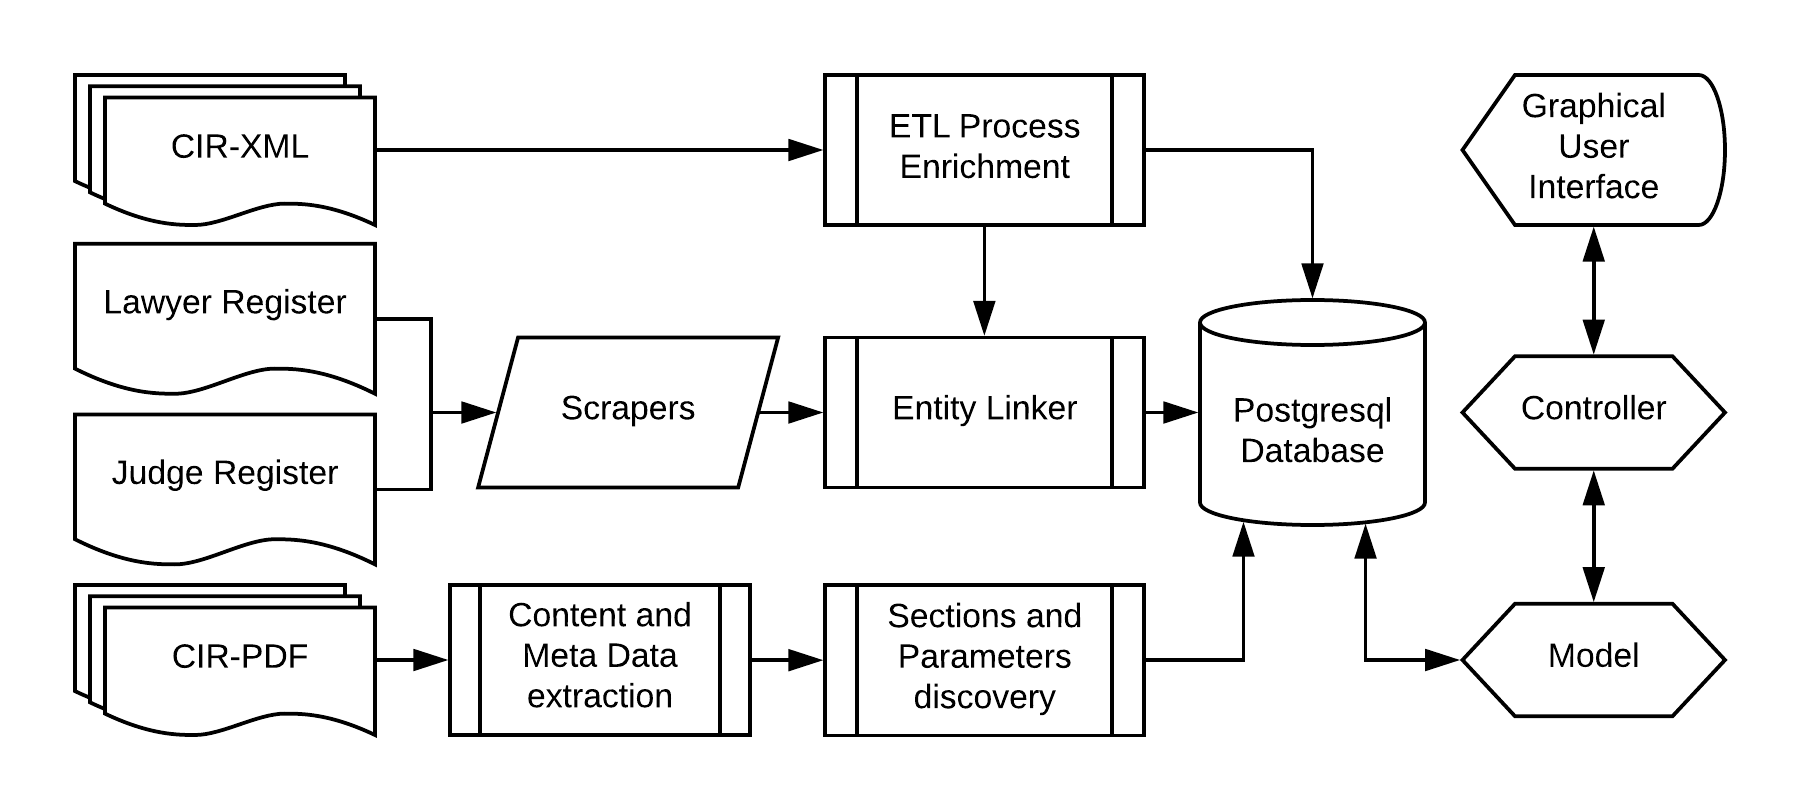
\includegraphics[width=1\linewidth]{images/system_overview.png}
\caption{System overview.}\label{System overview}
\end{figure}

Data flows from left to right through the following components:

\paragraph{Data Sources} Data is sourced from three public registers:
\begin{enumerate}
	\item The Central Insolvency Register (\textit{Centraal Insolventie Register or CIR}). CIR exposed both an XML and PDF file web service.
	\item The Register of lawyers (\textit{NOvA's Tableau}).
	\item The Register of ancillary positions of judges. (\textit{Register van nevenfuncties van rechters}) 
\end{enumerate}

The CIR provides the bulk of the data. The other two registers are used for the entity resolution of administrators and judges.

\paragraph{ETL and Enrichment} This component loads entities with selected data fields from the CIR XML data. The data is cleaned and enriched after which it is stored in a relational database.

\paragraph{Entity Linker} This component is responsible for linking judges and administrators in the CIR XML data to real life entities found in the judge and lawyer registers. 

\paragraph{PDF Processors}
These components processes the CIR PDF reports to extract textual content and meta data. The text sections as defined in the progress report template and key data parameter are discovered in a subsequent process and loaded into the relational database.

\paragraph{Database and File Storage}
Entity data is stored in a relational Postgresql database. Administrator PDF reports are stored in Amazon's S3 object storage.

\paragraph{Model-View-Controller (MVC)}
This well established pattern of subcomponents works together as a graphical interface for the user to analyse the data. 
%The user operates a graphical interface, prototyped in Jupyter notebooks, to query the data or interact with data visualisations or tables. The interface is the View in the MVC component. On user command, the Controller asks the Model to prepare the necessary data and then passes this data to the View to update the interface.
